\documentclass[a4paper, 10pt]{article}
\usepackage[T1]{fontenc}
\usepackage[utf8]{inputenc}
\usepackage[slovene]{babel}
\usepackage{lmodern}
\usepackage{amsmath}
\usepackage{leftidx}
\usepackage{amssymb}
\usepackage{amsfonts}
\usepackage{graphicx}
\usepackage{wrapfig}
\usepackage{amsthm}
\usepackage{mathrsfs}
\usepackage{mathtools}
\usepackage{url}
\usepackage{subfigure}
\usepackage{multirow}
\usepackage{lipsum}
\usepackage{wrapfig}
\usepackage{tikz}
\usepackage[format=plain, font=small, labelfont=bf, textfont=it, justification=centerlast]{caption}
\usepackage{booktabs}
\usepackage{siunitx}
\usepackage{enumerate}
\usepackage{ulem}
\usepackage{cancel}
\usepackage{algorithm2e}

\newtheorem{trditev}{Trditev}
\newtheorem{izr}{Izrek}
\newtheorem{nal}{Naloga}
\newtheorem{posl}{Posledica}

\newcounter{defcount}
\newcounter{opombe}
\newcounter{zgledcount}

\newenvironment{opomba}{\begin{flushleft}\stepcounter{opombe}\textbf{Opomba \arabic{opombe}:}}{\hfill\end{flushleft}}
\setlength{\parindent}{0mm}

\newenvironment{zgled}{\begin{flushleft}\stepcounter{zgledcount}\textbf{Zgled \arabic{zgledcount}:}}{\hfill\end{flushleft}}
\setlength{\parindent}{0mm}

\newenvironment{definicija}{\begin{flushleft}\stepcounter{defcount}\textbf{Definicija \arabic{defcount}:}}{\hfill\end{flushleft}}
\setlength{\parindent}{0mm}

\newenvironment{resitev}{\begin{flushleft}\textit{Rešitev:}}{\hfill\end{flushleft}}
\setlength{\parindent}{0mm}

\newcommand{\abs}[1]{\ensuremath{\lvert #1 \rvert}}
\newcommand{\mth}[1]{\ensuremath{\mathbb{#1}}}
\newcommand{\R}{\mth{R}}
\newcommand{\Z}{\mth{Z}}
\newcommand{\N}{\mth{N}}
\newcommand{\No}{\mth{N}_0}
\newcommand{\C}{\mth{C}}
\newcommand{\Cc}{\ensuremath{\mathcal{C}}}
\newcommand{\Dd}{\ensuremath{\mathcal{D}}}
\newcommand{\Mu}{\mathcal{M}}
\newcommand{\sigalg}{$\sigma$-algebra~}
\newcommand{\Qu}{\mth{Q}_u}

\newcommand{\pojem}[1]{\emph{#1}}
\newcommand{\Ob}[1]{\mathcal{O}b({#1})}
\newcommand{\Mor}[2][ ]{\mathcal{M}or_{#1}({#2})}
\newcommand{\con}{\ensuremath{\mathscr{C}}}
\newcommand{\padex}[2]{\ensuremath{{#1}^{\underline{#2}}}}
\newcommand{\rastx}[2]{\ensuremath{{#1}^{\bar{#2}}}}
\newcommand{\map}[3]{\ensuremath{{#1}: {#2} \rightarrow {#3}}}
\newcommand{\pra}[3]{{#1}{\ast}({#2}) = {#3}}

\title{Osnove programiranja v diskretni matematiki\\ Zapiski predavanj}
\date{2023/24}
%===============================================================================
\begin{document}
	\maketitle
	\newpage
	\begin{abstract}
		\noindent Dokument vsebuje zapiske predavanj predmeta Osnove programiranja v diskretni matematiki profesorja Vesela v okviru študija prvega letnika magistrskega študija matematike na FNM.
	\end{abstract}
	\tableofcontents
	\newpage
	\section{Predstavitve grafov in onsnovni algoritmi nad njimi}
	\begin{definicija}
		\pojem{Graf} $G$ je sestavljen iz množice ogljišč $V(G)$ in množice povezav $E(G)$. Pišemo: $G = (V, E)$. Pri tem pogosto označimo \abs{V}$=n$ in \abs{E}$=m$.
		Za $v\in V(G)$ definiramo $d(v) =~\textit{število sosed vozlišča $v$ v grafu}~G$
	\end{definicija}
	\begin{zgled} \label{zgl:grafG} Poglejmo si naslednji graf in v tabeli določimo vsakemu vozlišču njegove sosede. $G:$
		
		
		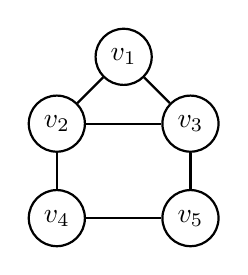
\begin{tikzpicture}[node distance = {12mm}, thick, main/.style = {draw, circle}]
			\node[main] (1) {$v_1$};
			\node[main] (2) [below left of=1] {$v_2$};
			\node[main] (3) [below right of=1] {$v_3$};
			\node[main] (4) [below of=2] {$v_4$};
			\node[main] (5) [below of=3] {$v_5$};
			
			\draw (1) -- (2);
			\draw (1) -- (3);
			\draw (2) -- (3);
			\draw (2) -- (4);
			\draw (3) -- (5);
			\draw (4) -- (5);
		\end{tikzpicture}
		
		\begin{table}[h!]
			\begin{tabular}{l|c|c|c|c|c|}
				Vozlišče & $v_1$ & $v_2$ & $v_3$ & $v_4$ & $v_5$ \\\hline
				Sosedi & $v_2, v_3$ & $v_1, v_3, v_4$ & $v_1, v_2, v_5$ & $v_2, v_5$ & $v_3, v_4$
			\end{tabular}
		\end{table}
	\end{zgled}
	Za predstavitev grafa imamo več možnosti. Prva možnost je matrika sosednosti, druga možnost (ki nas bo zanimala), pa so seznami sosedov. Seznami sosedov se izkažejo za bolj prostorsko varčne, saj matrika sosednosti tipično zavzame $O(n^2)$ mest, seznami sosedov pa manj. Koliko manj, je odvisno od načina implementacije.
	
	\subsection{Enostavni seznami sosedov}
	
	Sestavimo seznam $S$ vozlišč, tipično urejenih in oštevilčenih (npr $1$ predstavlja vozlišče $v_1$, $2$ vozlišče $v_2$ itd.). Nato sestavimo seznam sosedov $P$ tako, da po vrsti naštejemo sosede vozlišča $1$, nato vozlišča $2$, itd. Pri tem vsako vozlišče iz $S$ opremimo s kazalcem, ki kaže v $P$ na mesto, kjer se začnejo njegovi sosedi. 
	\begin{zgled}
		Predstavimo graf $G$ iz zgleda \ref{zgl:grafG} s pomočjo enostavnega seznama sosedov.
		\begin{table}[h!]
			$S$: \begin{tabular}{|c|c|c|c|c|}
				\hline
				$1$ & $2$ & $3$ & $4$ & $5$ \\\hline
			\end{tabular}
		\end{table}
		
		\begin{table}[h!]
			$P$: \begin{tabular}{|c|c||c|c|c||c|c|c||c|c||c|c|}
				\hline
				$2$ & $3$ & $1$ & $3$ & $4$ & $1$ & $2$ & $5$ & $2$ & $5$ & $3$ & $4$ \\\hline
			\end{tabular}
		\end{table}
	\end{zgled}
	Z $S_i$ označimo seznam sosedov vozlišča $v_i$. Seznam $S$ ima ravno $n$ mest, seznam $P$ pa $\sum_{i=1}^{n}d(v_i) = 2m$ mest. Prostorska zahtevnost enostavnih seznamov sosedov je torej $O(n + m)$, kar je po navadi res manj kot $O(n^2)$.
	\subsection{Razširjeni seznami sosedov}
	Najprej za vsako vozlišče $v_i$ sestavimo seznam sosedov $S_i$, v katerem vsakega od sosedov $v_i$ predstavimo s poljem $p$, ki je sestavljeno iz petih komponent: $p = (v_i, v_j, \&r, \&n, \&u)$. Pri tem je $v_i$ vozlišče, katerega sosede obravnavamo, $v_j$ ime soseda, $\&r$ kazalec, ki kaže na predhodnika $p$ v $S_i$, $\&n$ kazalec, ki kaže na naslednika $p$ v $S_i$ in $\&u$ kazalec, ki kaže na polje v seznamu $S_j$, ki predstavlja povezavo $v_iv_j$. Če je $p$ prvi v seznamu $S_i$ je $\&r = 0$, če je pa zadnji, je pa $\&n = 0$.
	
	\begin{zgled}
		\begin{table}[h!]
			\centering
			\begin{tabular}{|c|c|c|}
				Seznam & Ime polja & Polje \\\hline
				\multirow{2}{*}{$S_1$} & $a$ & $(v_1, v_2, 0, \&c, \&b)$ \\
				& $c$ & $(v_1, v_3, \&a, 0, \&d)$ \\\hline
				\multirow{3}{*}{$S_2$} & $b$ & $(v_2, v_1, 0, \&e, \&a)$ \\
				& $e$ & $(v_2, v_3, \&b, \&g, \&f)$ \\
				& $g$ & $(v_2, v_4, \&e, 0, \&h)$ \\\hline
				\multirow{3}{*}{$S_3$} & $d$ & $(v_3, v_1, 0, \&f, \&c)$ \\
				& $f$ & $(v_3, v_2, \&d, \&i, \&e)$ \\
				& $i$ & $(v_3, v_5, \&f, 0, \&j)$ \\\hline
				\multirow{2}{*}{$S_4$} & $h$ & $(v_4, v_2, 0, \&k, \&g)$ \\
				& $k$ & $(v_4, v_5, \&h, 0, \&l)$ \\\hline
				\multirow{2}{*}{$S_5$} & $j$ & $(v_5, v_3, 0, \&l, \&i)$ \\
				& $l$ & $(v_5, v_4, \&j, 0, \&k)$ \\\hline
			\end{tabular}
		\end{table}
	\end{zgled}
	Omenimo tukaj, da kadar grafu dodamo povezavo $v_iv_j$, to naredimo tako, da dodamo novo polje na začetek seznamov $S_i$ in $S_j$.
	\subsection{Časovna zahtevnost nekaterih operacij na grafih}
	Sedaj, ko smo uvedli različne sezname sosedov, lahko primerjamo časovno zahtevnost nekaterih klasičnih operacij na grafih.
	\begin{table}[h!]
		\centering
		\begin{tabular}{|c|c|c|}
			Operacija & Enostavni sez. & Razširjeni sez. \\\hline
			Preveri, če $G$ vsebuje povezavo $v_iv_j$ & $O(d(v_i))$ & $O(d(v_i))$ \\\hline
			Označi vse sosede vozlišča $v_i$ & $O(d(v_i))$ & $O(d(v_i))$ \\\hline
			Označi vse povezave & $O(m)$ & $O(m)$ \\\hline
			Dodaj povezavo $v_iv_j$ & $O(m)$ & $O(1)$ \\\hline
			Odstrani povezavo $v_iv_j$ & $O(m)$ & $O(d(v_i))$ \\\hline
			Odstrani vse povezave s krajiščem v $v_i$ & $O(m)$ & $O(d(v_i))$ \\\hline
		\end{tabular}
	\end{table}
	
	Izkaže se torej, da četudi imamo malenkost več dela z reprezentacijo grafov v razširjenih seznamih sosedov, s tem pridobimo na časovni zahtevnosti.
	
	\subsection{Urejanje seznamov sosedov}
	Za urejanje lahko, v splošnem, uporabimo algoritem z zahtevnostjo $O(k\log(k)$, kjer je $k$ število elementov seznama. Če to naredimo za vsak seznam dobimo: \begin{align*}
		\sum_{i=1}^{n} O(d(v_i)\log(d(v_i))) \leq \sum_{i=1}^{n} O(d(v_i)\log(n)) &= O(\log(n)\sum_{i=1}^{n}d(v_i)) \\
		&= O(m\log(n)) 
	\end{align*}
	To hitrost lahko torej pričakujemo pri enostavnih seznamih sosedov. Obstaja pa še hitrejši način, če si pomagamo z razširjenimi seznami sosedov. To naredimo tako, da upoštevamo, da je v vsakem polju seznama $S_i$ na v komponenti vozlišče $v_i$.
	Nove sezname gradimo tako, da se sprehajamo od seznama $S_n$, do $S_1$ in na vsakem koraku odstranimo polje $(v_i, v_j, \ldots)$ iz $S_i$. Nato odstranjenemu polju zamenjamo prvo in drugo komponento, da dobimo polje oblike $(v_j, v_i, \ldots)$ in to novo polje vstavimo na začetek novega seznama, ki ustreza vozlišču $v_j$. Algoritem še zapišemo bolj pregledno:
	\begin{algorithm}[h!]
		\KwData{Razširjeni seznami sosedov $S_1$,\ldots, $S_n$}
		\KwResult{Urejeni razširjeni seznami sosedov $B_1$,\ldots, $B_n$}
			Ustvari prazne razširjene sezname sosedov $B_1$,\ldots, $B_n$\;
			\For{i = n downto 1}{\While{$S_i\neq \emptyset$}{Odstrani prvo polje $p=(v_i, v_j, \ldots)$ iz $S_i$\; Dodaj $\acute{p} = (v_j, v_i, \ldots)$ na začetek $B_j$\;}}
	\end{algorithm}
		
		Ta algoritem ima časovno zahtevnost $O(m)$, torej je hitrejši od algoritma na enostavnih seznamih sosedov, katerih urejanje je imelo časovno zahtevnost $O(m\log(n))$.
	
\end{document}